\documentclass[a4paper]{article}
\usepackage[a4paper,margin=0mm]{geometry}
\usepackage{fontspec}
\usepackage{unicode-math}
\usepackage{tikz}
\usepackage[table]{xcolor}
\usepackage[absolute]{textpos}
\usepackage{enumitem}
\usepackage{array}
\usepackage{multirow}

\setmainfont{Libertinus Serif}
\setsansfont{Libertinus Sans}
\setmathfont{Libertinus Math}
\newfontfamily\trackedsans{Libertinus Sans}[LetterSpace=8.0]

\definecolor{accent}{HTML}{F46530}
\definecolor{badge}{HTML}{FFBDA5}
\definecolor{ink}{HTML}{2A2E30}

\setlength{\TPHorizModule}{1mm}
\setlength{\TPVertModule}{1mm}
\setlength{\parindent}{0pt}
\pagestyle{empty}

\newcommand{\LCOL}{16mm}
\newcommand{\RCOL}{111mm}
\newcommand{\COLW}{83mm}

\newcommand{\topicheader}[2]{%
\begin{textblock*}{194mm}(16mm,10mm)
\begin{tikzpicture}
\node[fill=accent,text=white,font=\sffamily\bfseries\fontsize{13}{13}\selectfont,
      minimum width=9mm,minimum height=9mm,inner sep=0pt] at (4.5mm,-4.5mm) {#1};
\node[font=\sffamily\bfseries\fontsize{15}{16}\selectfont,text=ink,anchor=west] at (12mm,-4.5mm) {#2};
\end{tikzpicture}
\end{textblock*}
\begin{textblock*}{194mm}(16mm,22.5mm)

\begin{tikzpicture}
\fill[accent] (0,0) rectangle (194mm,0.5mm);
\end{tikzpicture}
\end{textblock*}
}

\newcommand{\pagefooter}[1]{%
\begin{textblock*}{194mm}(8mm,286.41mm)
  
\begin{tikzpicture}
    \fill[accent] (0,0) rectangle (194mm,0.6mm);
  \end{tikzpicture}
\end{textblock*}
\begin{textblock*}{63.59mm}(8mm,288.27mm)
  {\sffamily\bfseries\color{accent}\fontsize{13}{16}\selectfont SAT 1200+}
\end{textblock*}
\begin{textblock*}{10mm}(188mm,288.27mm)
  \centering{\sffamily\color{accent}\fontsize{14}{16}\selectfont #1}
\end{textblock*}
}

\newcommand{\colrule}[2]{%
\begin{textblock*}{1mm}(105mm,#1mm)
\begin{tikzpicture}
\draw[black!65,line width=0.5pt] (0,0) -- (0,#2mm);
\end{tikzpicture}
\end{textblock*}
}

\newcommand{\setkicker}[2]{%
{\sffamily\bfseries\fontsize{12}{14}\selectfont #1.}\ {\itshape\fontsize{11}{14}\selectfont\color{black!75} #2}\par\vspace{2mm}%
}

\setlength{\fboxsep}{1.4pt}
\setlength{\fboxrule}{0.5pt}
\newcommand{\pnum}[1]{\fcolorbox{ink}{white}{\sffamily\bfseries\fontsize{8}{8}\selectfont #1}~}

\newcommand{\qrbox}[1]{%
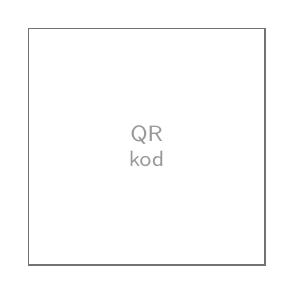
\begin{tikzpicture}
\draw[black!55,line width=0.6pt] (0,0) rectangle (30mm,30mm);
\node[black!40,font=\sffamily\fontsize{8}{9}\selectfont,align=center] at (15mm,15mm) {QR\\kod};
\end{tikzpicture}\\[1.5mm]
{\sffamily\fontsize{9}{11}\selectfont\color{black!70} #1}%
}

\arrayrulecolor{accent}
\setlength{\arrayrulewidth}{0.7pt}
\renewcommand{\arraystretch}{1.35}
\newcommand{\anstitle}[1]{{\sffamily\bfseries\color{accent}\fontsize{11}{13}\selectfont #1}\\[1.3mm]}

\begin{document}

% ================= PAGE 1: Set 1 | Set 2 =================
\topicheader{13}{Nisbat, tezlik va proportsiya}
\pagefooter{1}
\colrule{32}{238}
\mbox{}%

\begin{textblock*}{\COLW}(\LCOL,32mm)
{\fontsize{12}{15}\selectfont
\setkicker{1-to'plam}{Nisbatni eng sodda ko'rinishga keltiring.}

\noindent\pnum{1} $10:15$ nisbatini eng sodda ko'rinishga keltiring.\\[20mm]
\noindent\pnum{2} $21:14$ nisbatini eng sodda ko'rinishga keltiring.\\[20mm]
\noindent\pnum{3} $16:24:40$ nisbatini eng sodda ko'rinishga keltiring.\\[20mm]
\noindent\pnum{4} Qutida $9$ ta qizil va $12$ ta ko'k shar bor. Qizil:ko'k nisbatini eng sodda ko'rinishda yozing.\\[22mm]
\noindent\pnum{5} $24$ ni $36$ ga nisbatini eng sodda ko'rinishda yozing.\\[20mm]
\noindent\pnum{6} Nisbat $4:9$. Jami nechta ``qism'' bor?
}
\end{textblock*}

\begin{textblock*}{\COLW}(\RCOL,32mm)
{\fontsize{11.5}{15}\selectfont
\setkicker{2-to'plam}{Qism-qismga va qism-butunga nisbat -- avval jami qismlar sonini toping.}

\noindent\pnum{1} Sinfda o'g'il:qiz nisbati $3:5$, jami $40$ o'quvchi. Nechta o'g'il bola bor?\\[18mm]
\noindent\pnum{2} Yuqoridagi sinfda: qiz bolalar butunning qanday qismini tashkil qiladi?\\[18mm]
\noindent\pnum{3} Mushuk:it nisbati $2:7$, jami $27$ ta uy hayvoni. Nechta it bor?\\[18mm]
\noindent\pnum{4} Qizil:ko'k shar nisbati $4:5$, jami $36$ ta shar. Qizil sharlar butunning qanday qismi?\\[20mm]
\noindent\pnum{5} Olma:apelsin nisbati $5:3$, jami $32$ ta meva. Olmalar apelsinlardan nechta ko'p?\\[18mm]
\noindent\pnum{6} Un:shakar nisbati $5:2$, jami $70$ stakan. Nechta stakan shakar kerak?
}
\end{textblock*}

\clearpage

% ================= PAGE 2: Set 3 | Set 4 =================
\topicheader{13}{Nisbat, tezlik va proportsiya}
\pagefooter{2}
\colrule{32}{238}
\mbox{}%

\begin{textblock*}{\COLW}(\LCOL,32mm)
{\fontsize{12}{15}\selectfont
\setkicker{3-to'plam}{Tezlik va birlik tezlik.}

\noindent\pnum{1} Mashina $3$ soatda $180$ km yuradi. Birlik tezlikni (km/soat) toping.\\[20mm]
\noindent\pnum{2} Fabrika $5$ soatda $250$ dona ishlab chiqaradi. Soatiga nechta dona?\\[20mm]
\noindent\pnum{3} $15$ kg guruch $45$ dollar turadi. $1$ kg narxi qancha?\\[20mm]
\noindent\pnum{4} Printer $4$ daqiqada $48$ bet chop etadi. Daqiqasiga nechta bet?\\[20mm]
\noindent\pnum{5} Qaysi tezlik kattaroq: $2$ soatda $120$ milya, yoki $3$ soatda $150$ milya?\\[20mm]
\noindent\pnum{6} Yuguruvchi $50$ soniyada $400$ metr yuguradi. Soniyasiga necha metr?
}
\end{textblock*}

\begin{textblock*}{\COLW}(\RCOL,32mm)
{\fontsize{12}{15}\selectfont
\setkicker{4-to'plam}{Proportsiyani yeching va masshtablang.}

\noindent\pnum{1} $\dfrac{x}{5} = \dfrac{12}{20}$ tenglamasini yeching.\\[20mm]
\noindent\pnum{2} $\dfrac{8}{x} = \dfrac{6}{15}$ tenglamasini yeching.\\[20mm]
\noindent\pnum{3} $\dfrac{3}{4} = \dfrac{x}{28}$ tenglamasini yeching.\\[20mm]
\noindent\pnum{4} Retseptda un:shakar $=3:5$. $18$ stakan un bo'lsa, nechta stakan shakar kerak?\\[20mm]
\noindent\pnum{5} Xarita masshtabi: $1$ dyuym $=15$ milya. $4.5$ dyuym necha milya?\\[20mm]
\noindent\pnum{6} Xarita masshtabi: $2$ sm $=25$ km. $7$ sm necha km?
}
\end{textblock*}

\clearpage

% ================= PAGE 3: Set 5 | Set 6 (spot the error) =================
\topicheader{13}{Nisbat, tezlik va proportsiya}
\pagefooter{3}
\colrule{32}{238}
\mbox{}%

\begin{textblock*}{\COLW}(\LCOL,32mm)
{\fontsize{11.5}{15}\selectfont
\setkicker{5-to'plam}{Aralash masalalar.}

\noindent\pnum{1} Tadbirda erkak:ayol nisbati $5:3$, jami $96$ kishi. Erkaklar ayollardan nechta ko'p?\\[18mm]
\noindent\pnum{2} Mashina har $28$ milyaga $1$ gallon benzin sarflaydi. $182$ milya uchun necha gallon kerak?\\[20mm]
\noindent\pnum{3} O'qituvchi:o'quvchi nisbati $1:18$. $36$ ta o'qituvchi bo'lsa, nechta o'quvchi bor?\\[18mm]
\noindent\pnum{4} Pons retseptida sharbat:soda nisbati $4:3$. Jami $56$ stakan uchun nechta stakan soda kerak?\\[20mm]
\noindent\pnum{5} Mashina $5$ daqiqada $60$ shisha to'ldiradi. Shu tezlikda $192$ shishaga necha daqiqa kerak?\\[18mm]
\noindent\pnum{6} Jamg'arma:xarajat nisbati $2:5$. $350$ dollar sarflansa, qancha pul jamg'ariladi?
}
\end{textblock*}

\begin{textblock*}{\COLW}(\RCOL,32mm)
{\fontsize{10.3}{13}\selectfont
\setkicker{6-to'plam}{Xatoni toping -- buzilgan qadamni ayting, to'g'ri javobni bering.}

\noindent\pnum{1} Qizil:ko'k nisbati $3:7$, jami $50$ shar. Xato yechim:\\[1mm]
\hspace*{7mm}\textit{``Qizil $= \frac{3}{7}\times50 \approx 21.43$.''}\\[2mm]
\hspace*{7mm}Xato va to'g'ri javob: \makebox[52mm]{\dotfill}\\[6mm]

\noindent\pnum{2} $\dfrac{x}{6}=\dfrac{10}{15}$. Xato yechim:\\[1mm]
\hspace*{7mm}\textit{``Ko'ndalang: $x\times10=6\times15$, $10x=90$, $x=9$.''}\\[2mm]
\hspace*{7mm}Xato va to'g'ri javob: \makebox[52mm]{\dotfill}\\[6mm]

\noindent\pnum{3} Poezd $2$ soat $30$ daqiqada $120$ km. Xato yechim:\\[1mm]
\hspace*{7mm}\textit{``Tezlik $=120\div2=60$ km/soat.''}\\[2mm]
\hspace*{7mm}Xato va to'g'ri javob: \makebox[52mm]{\dotfill}\\[6mm]

\noindent\pnum{4} Qalam:ruchka $4:9$, $36$ ta ruchka. Xato yechim:\\[1mm]
\hspace*{7mm}\textit{``$\frac{4}{9}=\frac{36}{p}$, $4p=324$, $p=81$.''}\\[2mm]
\hspace*{7mm}Xato va to'g'ri javob: \makebox[52mm]{\dotfill}\\[6mm]

\noindent\pnum{5} $5$ ta daftar $20$ dollar. Xato yechim:\\[1mm]
\hspace*{7mm}\textit{``Birlik tezlik $=\frac{5}{20}=0.25$ dollar.''}\\[2mm]
\hspace*{7mm}Xato va to'g'ri javob: \makebox[52mm]{\dotfill}
}
\end{textblock*}

\clearpage

% ================= PAGE 4: Set 7 (bonus) =================
\topicheader{13}{Nisbat, tezlik va proportsiya}
\pagefooter{4}
\colrule{32}{238}
\mbox{}%

\begin{textblock*}{\COLW}(\LCOL,32mm)
{\fontsize{11.5}{15}\selectfont
\setkicker{7-to'plam}{Bonus / qiyin -- 2+ qadamli masalalar.}

\noindent\pnum{1} Davlat yutgan oltin:kumush:bronza nisbati $2:3:4$, jami $54$ medal. Bronza oltindan nechta ko'p?\\[22mm]
\noindent\pnum{2} Fabrika $4$ soatda $180$ dona ishlab chiqaradi. $540$ dona uchun necha soat kerak?\\[22mm]
\noindent\pnum{3} Xarita masshtabi: $3$ sm $=40$ km. $150$ km necha santimetr?\\[22mm]
\noindent\pnum{4} Aziz:Bekzod yoshi hozir $3:4$. $5$ yil oldin bu nisbat $2:3$ edi. Hozirgi yoshlarini toping.\\[24mm]
\noindent\pnum{5} Mashina $2$ soat $60$ milya/soat, keyin $3$ soat $45$ milya/soat tezlikda yuradi. Butun sayohat uchun o'rtacha tezlikni toping.
}
\end{textblock*}

\clearpage

% ================= PAGE 5: Javoblar -- full-page answer tables, own page always =================
\topicheader{13}{Nisbat, tezlik va proportsiya}
\pagefooter{5}
\mbox{}%

\begin{textblock*}{194mm}(16mm,30mm)
{\bfseries\itshape\color{accent}\fontsize{19}{21}\selectfont\centering Javoblar\par}
\end{textblock*}

\begin{textblock*}{194mm}(16mm,44mm)
{\fontsize{9.3}{11.8}\selectfont
\centering
\renewcommand{\arraystretch}{1.3}
\begin{tabular}{|>{\centering\arraybackslash}p{26mm}|>{\centering\arraybackslash}p{10mm}|>{\centering\arraybackslash}p{32mm}|>{\centering\arraybackslash}p{10mm}|>{\centering\arraybackslash}p{32mm}|}
\hline
\rowcolor{badge!55}\textbf{To'plam} & \textbf{\#} & \textbf{Javob} & \textbf{\#} & \textbf{Javob}\\
\hline
\multirow{3}{26mm}{\centering 1-to'plam} & 1 & $2:3$ & 2 & $3:2$\\\cline{2-5}
 & 3 & $2:3:5$ & 4 & $3:4$\\\cline{2-5}
 & 5 & $2:3$ & 6 & $13$\\\hline
\multirow{3}{26mm}{\centering 2-to'plam} & 1 & 15 o'g'il & 2 & $\frac{5}{8}$\\\cline{2-5}
 & 3 & 21 it & 4 & $\frac{4}{9}$\\\cline{2-5}
 & 5 & 8 ta ko'p & 6 & 20 stakan\\\hline
\multirow{3}{26mm}{\centering 3-to'plam} & 1 & 60 km/soat & 2 & 50/soat\\\cline{2-5}
 & 3 & \$3/kg & 4 & 12 bet/daq\\\cline{2-5}
 & 5 & 1-chisi (60mph) & 6 & 8 m/s\\\hline
\multirow{3}{26mm}{\centering 4-to'plam} & 1 & $x=3$ & 2 & $x=20$\\\cline{2-5}
 & 3 & $x=21$ & 4 & 30 stakan\\\cline{2-5}
 & 5 & 67.5 milya & 6 & 87.5 km\\\hline
\multirow{3}{26mm}{\centering 5-to'plam} & 1 & 24 ko'p & 2 & 6.5 gal\\\cline{2-5}
 & 3 & 648 o'q. & 4 & 24 stakan\\\cline{2-5}
 & 5 & 16 daq & 6 & \$140\\\hline
\multirow{3}{26mm}{\centering 7-to'plam} & 1 & 12 ko'p & 2 & 12 soat\\\cline{2-5}
 & 3 & 11.25 sm & 4 & 15 \& 20 yosh\\\cline{2-5}
 & 5 & 51 mph & -- & --\\\hline
\multirow{5}{26mm}{\centering 6-to'plam} & \multicolumn{4}{p{82mm}|}{1.\ Xato -- qism-qismga va qism-butunga nisbatni aralashtirgan. To'g'ri: $\frac{3}{10}\times50=15$.}\\\cline{2-5}
 & \multicolumn{4}{p{82mm}|}{2.\ Xato -- ko'ndalang ko'paytirishda noto'g'ri juftlik. To'g'ri: $15x=60$, $x=4$.}\\\cline{2-5}
 & \multicolumn{4}{p{82mm}|}{3.\ Xato -- $30$ daqiqani soatga aylantirmagan. To'g'ri: $120\div2.5=48$ km/soat.}\\\cline{2-5}
 & \multicolumn{4}{p{82mm}|}{4.\ Xato -- proportsiya tartibini aralashtirgan. To'g'ri: $9p=144$, $p=16$.}\\\cline{2-5}
 & \multicolumn{4}{p{82mm}|}{5.\ Xato -- birlik tezlikni teskari hisoblagan. To'g'ri: $20\div5=4$ dollar/daftar.}\\\hline
\end{tabular}
}
\end{textblock*}

\begin{textblock*}{194mm}(16mm,232mm)
\centering
{\sffamily\fontsize{9.5}{11.5}\selectfont\color{black!70} Video yechimlar va qo'shimcha testlar uchun quyidagi QR kodlarni skanerlang:}\\[4mm]
\begin{minipage}[t]{32mm}\centering\qrbox{YouTube}\end{minipage}%
\hspace{16mm}%
\begin{minipage}[t]{32mm}\centering\qrbox{Telegram}\end{minipage}
\end{textblock*}

\end{document}
